% 固定来源 PDF 印刷页 87 第 21 题评分解析辅助构造示意重绘。
% 在原题关系上增加 E 为 DC 中点、Q 为 DP 中点以及连接线；投影不表示度量比例。
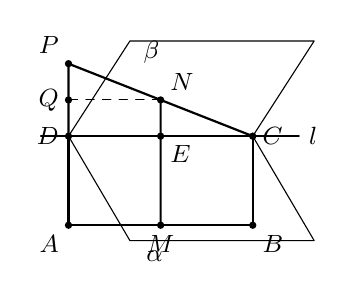
\begin{tikzpicture}[scale=.78,font=\small,line cap=round,line join=round]
  \coordinate (D) at (1,0);
  \coordinate (C) at (4,0);
  \coordinate (A) at (1,-1.45);
  \coordinate (B) at (4,-1.45);
  \coordinate (P) at (1,1.18);
  \coordinate (M) at (2.5,-1.45);
  \coordinate (N) at (2.5,.59);
  \coordinate (E) at (2.5,0);
  \coordinate (Q) at (1,.59);
  \draw[thin] (D)--(C)--(5,-1.7)--(2,-1.7)--cycle;
  \draw[thin] (D)--(C)--(5,1.55)--(2,1.55)--cycle;
  \draw[thick] (.55,0)--(4.75,0) node[right] {$l$};
  \node at (2.4,-1.95) {$\alpha$};
  \node at (2.35,1.37) {$\beta$};
  \draw[thick] (A)--(B)--(C)--(D)--cycle;
  \draw[thick] (P)--(A) (P)--(C) (M)--(N);
  \draw[dashed] (M)--(E) (N)--(E) (N)--(Q) (A)--(Q);
  \fill (A) circle (1.7pt) node[below left] {$A$};
  \fill (B) circle (1.7pt) node[below right] {$B$};
  \fill (C) circle (1.7pt) node[right] {$C$};
  \fill (D) circle (1.7pt) node[left] {$D$};
  \fill (P) circle (1.7pt) node[above left] {$P$};
  \fill (M) circle (1.7pt) node[below] {$M$};
  \fill (N) circle (1.7pt) node[above right] {$N$};
  \fill (E) circle (1.7pt) node[below right] {$E$};
  \fill (Q) circle (1.7pt) node[left] {$Q$};
\end{tikzpicture}
